\section{Edmonds-Karp}
In 1972 Edmonds and Karp published a paper detailing a specific protocol using the Ford-Fulkerson method for computing max flow and min cut. The Edmonds-Karp (EK) algorithm is one of the earliest solutions for solving the maximum flow in a network of nodes that can be represented as a graph. Unlike its predecessor, it has a well defined specification on how to perform searches for augmenting paths. While Ford-Fulkerson may use any search method, often DFS, EK requires the use of BFS to find augmenting paths which improves theoretical runtimes from $\mathcal{O}(E|f|)$, where $f$ is the max flow of the graph, to $\mathcal{O}(V^2E)$.

\subsection{Sequential Algorithm}
In order to test our parallel algorithm on correctness and speed, we implemented the EK algorithm in Java by editing an existing version of the algorithm written by one of our fellow classmates, Pedro Contepelli, who has given us full permission to use and edit his code for our research as needed. The algorithm uses three different classes to maintain a graph (\textit{Graph}), its edges (\textit{Edge}), and its nodes (\textit{Node}).  
    
A \textit{Graph} is instantiated from a text based input file holding the matrix representing the graph and the number of \textit{Node}s it has. The Source and the Sink are assumed to be $0$ and $n-1$ respectively. The \textit{Graph} also has a method \textit{getAugPath()} which returns an augmenting path in the graph.

From there \textit{main()} runs the EK algorithm to compute the max flow for the graph. It does this by finding the maximum flow that can be pushed through the obtained path and then adds each edge's flow to the forward flow of the edge and subtracts it from the reverse flow of the edge. It should be noted that this algorithm is also useful in solving the min-cut problem as well as the max flow problem because they are both the same problem [Ford-Fulkerson].
    
\subsection{Parallel Algorithm}
We believe there are two distinct ways to transform the sequential Edmonds-Karp algorithm into a version that applies some concurrency to the algorithm. The first is strictly through parallelization of the BFS algorithm to decrease the augmenting paths search time, and the second is by using fine-grained locking techniques to build augmenting paths in parallel using several threads running BFS concurrently on a single graph data structure. We will discuss each approach and explain why we chose attempt to build a concurrent graph using Java's parallel libraries.
    
\subsubsection{Parallel Breadth-First-Search}
Implementing a parallel BFS was the first thought that came to mind when attempting to create a parallel implementation of the EK algorithm. BFS is an incredibly time intensive task running in $\mathcal{O}(V+E)$ time while the rest of the algorithm simply adds a multiple of the BFS run time because calculations are performed on the path BFS finds. If we could speedup the search rate for an augmenting path then we could potentially see impressive gains in speedup for the overall EK algorithm. Taking this approach would prove difficult, however, as other research says that BFS is not easily parallelizable which lead us to parallelization \cite{vineet}.

\subsubsection{Parallel Augmenting Paths}
It is possible to allow multiple threads to try to update the graph based on the augmenting path they have found. There are two possible ways to handle these graph updates in a concurrent environment. We could use coarse-grained locks on the graph data structure while the flows and capacities are being updated to ensure mutual exclusion. This approach could produce significantly less speedup than desired due to the locks potentially forcing the program into a sequential state. Another option would be to create a fine-grained locking system that only locks the current augmented path edges while they are being updated.   

Using a coarse-grained lock would allow BFS computations for augmenting paths to be done in parallel while locking the calculations necessary to update the flows and capacities of each of the edges in the augmenting path. Unfortunately, this method would not be particularly useful because each augmenting path found in parallel would then be discarded when one of the threads successfully updates the graph. This parallel version would be significantly easier to write than implementing a parallel BFS, but could lead to the algorithm being nearly sequential as mentioned earlier so we will try another method.

Applying fine-grained locking techniques to the \textit{Graph} will allow it to become a more versatile concurrent data structure. Instead of refusing access to the entire \textit{Graph} we can simply lock the parts of the graph that we need to perform calculations on, namely the path generated by BFS, while other threads are free to perform work on parts of the \textit{Graph} that have not yet been locked.

\subsubsection{Fine-Grained Concurrent Graph Initial Approach}
To build a fine-grained concurrent data structure we have to take careful consideration in how we implement each field and method associated with the object. For the parallel EK algorithm we will need to create a shared memory \textit{Graph} that is capable of being searched by several threads and then having updates to the residual capacities and flows of those paths applied in parallel. To achieve this we will lock each edge of the augmenting path as it is being added to our augmenting path variable to ensure no other threads try to make residual capacity or flow updates to the edges in the current thread's augmenting path. In short, we need to add a lock to \textit{Edge} and require threads to acquire this \textit{Edge}'s lock before continuing. We define the specifications we think are required to create a concurrent \textit{Graph} in pseudo code in the Algorithm \ref{EKClassesInitial}

As described, the function locks the edges of the path as it builds it so that other threads cannot try to access the same $ConcurrentEdge$ at the same time. These classes are very specific to the EK algorithm and require the $run$ method to be run to for each of these class methods to work properly, specifically the $getAugmentingPath$ method relies on the $edmondsKarp$ method from Algorithm \ref{EKP} to unlock each $ConcurrentEdge$ in the path before starting another BFS.

\subsubsection{Fine-Grained Concurrent Graph Final Approach}
Through some preliminary testing it was clear that the initial approach had some efficiency short comings. After analyzing the algorithm, it is clear that there is a path bottleneck, especially for smaller graphs. In larger graphs, as each thread builds a path the only thing that will cause delay is colliding with another path. The current algorithm is naive and waits for its desired path to become available which undoubtedly increases the run time. This can be mended by requeuing the locked edge and moving on to the next available edge in the queue so as not to delay progress and to also not miss out on any possible paths. It is possible that all edges that a thread wants to acquire are locked, but this scenario is far less likely to happen so significant speedup is expected. This requires a change to the $getAugmentingPaths$ function in \textit{Concurrent Classes} which can be observed in the pseudocode Algorithm \ref{EKClassesFinal}. There are no necessary changes to the overall Edmonds-Karp algorithm described in Algorithm \ref{EKP}.

\subsection{Testing \& Results}
\vspace{7}
    These test results were performed on UCF's Eustis3 server utilizing open-source data sets \cite{sumitpadhiyar} running on eight threads. The results on the table are an average of 3 runs.
    
    It can be seen from the table the the initial parallel approach performed worse than its sequential counterpart. For the sake of time, the ten thousand node test was foregone for the initial approach. After some analysis of the algorithm it became clear that, while having the correct solution, it would be much slower than the sequential version due to the overhead of running eight threads. This was the inspiration for finding the final approach to the parallelization of the Edmonds-Karp algorithm.
    
    The final approach algorithm performed better than the initial approach overall as expected. Interestingly, for graphs with less than 1000 nodes, the final approach algorithm was slower than the initial approach. This could be because of the sparsity of the test graph, but is undetermined.
    
    \begin{table}[h]
    \centering
        \begin{tabular}{ | m{3em} | m{4em}| m{5em} | m{4em} | m{4em}|}
          \hline
          Nodes & Max Flow & Sequential Time & Initial Parallel Time & Final Parallel Time \\ 
          
            \hline
            50      & 828     & 3ms & 11ms & 36 ms\\
            \hline
            100     & 1251    & 11ms & 22ms & 79ms\\  
            \hline
            500     & 7143    & 123ms & 403ms & 604ms\\        
            \hline   
            750     & 10930   & 253ms & 1456ms & 1656ms\\         
            \hline
            1000    & 13476   & 1227ms & 3968ms & 3467ms\\       
            \hline
            2000    & 25027   & 8837ms & 39514ms & 23382ms\\
            \hline
            3000    & 39170   & 32302ms & 117157ms & 82435ms\\       
            \hline
            4000    & 58517   & 78587ms & 307633ms & 210706ms\\
            \hline
            5000    & 69349   & 142469ms & 575808ms & 387658ms\\
            \hline
            10000   & 142610  & 1189164ms & N/A & N/A\\
            \hline
        \end{tabular}
    \end{table}
    The final 10,000 node test could not be completed due to not enough heap space. Unfortunately, neither attempt at parallelization was able to improve the run time when compared with the sequential algorithm. This may be due to the structure of the graph being an adjacency list rather than an adjacency matrix. Future research might consider this idea.
\begin{figure}
    \hspace{-20}
    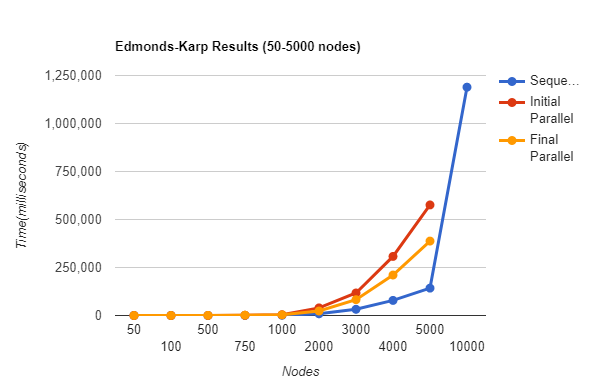
\includegraphics[scale=0.48]{figures/ek-line.png}
    \label{fig:my_label}
\vspace{-9}
\end{figure}


    
\begin{algorithm}
\caption{Initial Concurrent Classes}
\label{EKClassesInitial}
    \begin{algorithmic}[1]
    \State \textbf{class} $ConcurrentGraph$ \\
        \Function{$getAugmentingPath$}{}
            \State $path \gets$ array of $Edges$
            \State $queue \gets$ empty queue of $Nodes$
            \State add source node to $queue$
            \While {$queue$ is not empty}
                \State remove node from $queue$
                \For{each edge in the current node}
                    \If{meets augmenting path requirements}
                        \State try to acquire edge lock
                        \State add edge to augmenting path
                        \State add node connected to edge to $queue$
                    \EndIf
                \EndFor
            \EndWhile
        \EndFunction
    \\
    \State \textbf{class} $ConcurrentEdge$
        \State $u \gets$ integer
        \State $v \gets$ integer
        \State $flow \gets$ integer
        \State $capacity \gets$ integer
        \State $reverse \gets Edge$
        \State $lock \gets$ reentrant lock
        \Function{lock}{}
            \State \textbf{do} $lock$.lock
        \EndFunction
        \Function{unlock}{}
            \State \textbf{do} $lock$.unlock
        \EndFunction
    \end{algorithmic}   
\end{algorithm}

\begin{algorithm} 
\caption{Edmonds-Karp Parallel Implementation}
\label{EKP}
    \begin{algorithmic}[1]
    \Function{$edmondsKarp$}{}
        \State $graph \gets$ constructor creates graph from file
        \State $maxFlow \gets$ integer
        \While{true}
            \State $path \gets getAugmentingPath$
            \If{$path$ does not contain the sink}
                \Return
            \Else
                \State $forwardFlow \gets INFINITY$
                \For{each $ConcurrentEdge$ in $path$}
                    \State $forwardFlow \gets$ minimum residual flow
                \EndFor
                \For{each $ConcurrentEdge$ in $path$}
                    \State add $forwardFlow$ to $flow$
                    \State{subtract $forwardFlow$ from $reverseFlow$}
                \EndFor
                \State $maxFlow \gets maxFlow + pushFlow$
                \For{each $ConcurrentEdge$ in $path$}
                    \State \textbf{do} $ConcurrentEdge.lock$.unlock
                \EndFor
            \EndIf
        \EndWhile
    \EndFunction
    \end{algorithmic}
\end{algorithm}

\begin{algorithm} 
\caption{Final Concurrent Classes}
\label{EKClassesFinal}
    \begin{algorithmic}[1]
        \Function{$getAugmentingPath$}{}
            \State $path \gets$ array of $Edges$
            \State $queue \gets$ empty queue of $Nodes$
            \State add source node to $queue$
            \While {$queue$ is not empty}
                \State remove node from $queue$
                \State $edgeQ \gets$ queue of $Edges$ 
                \For{each edge in the current node}
                    \If{meets augmenting path requirements}
                        \State try to acquire edge lock
                        \If{successful}
                            \State add edge to augmenting path
                            \State add node connected to edge to $queue$
                        \Else
                            \State add edge to $edgeQ$
                        \EndIf
                    \EndIf
                \EndFor
                \While {$edgeQ$ is not empty}
                    \State $Edge e \gets$ $edgeQ$.poll
                    \If{meets augmenting path requirements}
                        \State try to acquire edge lock
                        \If{successful}
                            \State add edge to augmenting path
                            \State add node connected to edge to $queue$
                        \Else
                            \State add edge to $edgeQ$
                        \EndIf
                    \EndIf
                \EndWhile        
            \EndWhile
        \EndFunction
    \end{algorithmic}   
\end{algorithm}

\clearpage